\documentclass[11pt,a4paper,notitlepage]{exam}
\usepackage[utf8]{inputenc}
\usepackage{graphicx, wrapfig}

\usepackage{amsmath}
\usepackage{amsthm}
\usepackage{amssymb}
\usepackage{mathtools}
\usepackage[shortlabels]{enumitem}

\renewcommand*{\proofname}{Prova}
% bold math
\usepackage{amsbsy}

% draw pictures (and graphs)
\usepackage{tikz}

% \usepackage[usenames,dvipsnames,svgnames,table]{xcolor}

% code in latex
\definecolor{dkgreen}{rgb}{0,0.6,0}
\definecolor{gray}{rgb}{0.5,0.5,0.5}
\definecolor{mauve}{rgb}{0.58,0,0.82}
\definecolor{newink}{rgb}{0,0.1,0.25}
\usepackage{caption}
\usepackage{listings}
\lstset{frame=tb,
  language=Python,
  aboveskip=3mm,
  belowskip=3mm,
  showstringspaces=false,
  columns=flexible,
  basicstyle={\small\ttfamily},
  numbers=none,
  numberstyle=\tiny\color{gray},
  keywordstyle=\color{blue},
  commentstyle=\color{dkgreen},
  stringstyle=\color{mauve},
  breaklines=true,
  breakatwhitespace=true,
  tabsize=3
}


\usepackage{multirow}

% definition equal
\newcommand\eqdef{\mathrel{\overset{\makebox[0pt]{\mbox{\normalfont\tiny\sffamily def}}}{=}}}

% independence equal
\newcommand\eqindep{\mathrel{\overset{\makebox[0pt]{\mbox{\normalfont\tiny\sffamily indep}}}{=}}}


% independent and identically distributed equal
\newcommand\eqiid{\mathrel{\overset{\makebox[0pt]{\mbox{\normalfont\tiny\sffamily i.i.d.}}}{=}}}

% * to cdot
% \mathcode`\*="8000
% {\catcode`\*\active\gdef*{\cdot}}
\usepackage[table,xcdraw]{xcolor}
% pseudo-code
\usepackage[portuguese, linesnumbered]{algorithm2e}
\newcommand\Recebe{\leftarrow}
\newcommand\Comment{\vartriangleright}
\SetKw{Devolva}{devolva}
% Example:
% \paragraph{}
% \SetAlgoNoLine
% \textsc{Título-Do-Algoritmo}($A, n$)\\
% \begin{algorithm}[H]
%   \Devolva $A$
% \end{algorithm}
%

% pair ceil
\DeclarePairedDelimiter{\ceil}{\lceil}{\rceil}

% pair ceil
\DeclarePairedDelimiter{\floor}{\lfloor}{\rfloor}

% images
\usepackage{graphicx}
\graphicspath{ {./} }
% use: \includegraphics[scale=1]{image}


\setlength{\parindent}{3em}
\setlength{\parskip}{0.5em}

\usetikzlibrary{graphs,graphs.standard}

\newcount\nodecount
\tikzgraphsset{
  declare={subgraph N}%
  {
    [/utils/exec={\global\nodecount=0}]
    \foreach \nodetext in \tikzgraphV
    {  [/utils/exec={\global\advance\nodecount by1}, 
      parse/.expand once={\the\nodecount/\nodetext}] }
  },
  declare={subgraph C}%
  {
    [cycle, /utils/exec={\global\nodecount=0}]
    \foreach \nodetext in \tikzgraphV
    {  [/utils/exec={\global\advance\nodecount by1}, 
      parse/.expand once={\the\nodecount/\nodetext}] }
  }
}
\linespread{1.2}

\begin{document}
% \SetAlgoNoLine
\begin{center}
    %NOME E NUSP
    Nome: Rogério Marcos Fernandes Neto\hphantom{xxx} NUSP: 10284632\\
    %CURSO
    Curso: Bacharelado em Ciência da Computação\\
    %MATÉRIA
    MAC0320 - Introdução à Teoria dos Grafos
    \paragraph{}
    \textbf{LISTA 10}
\end{center}
    \paragraph{E39.} Mostre que se $G$ é um grafo simples conexo planar
    com cintura $k \geq 3$, então 
    $$
        |A(G)| \leq k(|V(G)| -2)/(k-2)
    $$
    Usando o resultado acima prove que o grafo de Petersen não é planar.
    (Lembramos que a \textit{cintura} de $G$ é o comprimento de um menor
    circuito de $G$.)
    \paragraph{Solução:}
    \begin{proof}
        Seja $G$ um grafo simples conexo com cintura $k \geq 3$.\par
        Note que nesse grafo temos que $gr(f) \geq k$. De fato, como
        $n\geq k$ então a face externa deve ter no mínimo grau k (caso
        onde não existem arestas de corte), e, como $G$ é
        simples, qualquer outra face é determinada por um circuito
        facial, e cada circuito dessa forma tem grau no mínimo $k$.
        Portanto, temos que
        $$
        k|F(G)| \leq \sum_{f \in F(G)}gr(f)
        $$
        Pelo \textbf{teorema 9.1} sabemos que $\sum_{f \in F(G)}gr(f) =
        2|A(G)|$. Portanto
        $$
        k|F(G)| \leq 2|A(G)|
        $$
        Além disso, sabemos pela \textbf{fórmula de Euler} que $|F(A)| =
        2 +  |A(G)| - |V(G)|$. Assim, temos que
        \begin{align*}
            k(2 +  |A(G)| - |V(G)|) &\leq 2|A(G)|\\
            2k + |A(G)|k - |V(G)|k &\leq 2|A(G)|\\
            |A(G)|k + 2|A(G)| &\leq |V(G)|k - 2k\\
            |A(G)|(k-2) &\leq k(|V(G)| - 2)\\
            |A(G)| &\leq \dfrac{k(|V(G)| - 2)}{(k-2)}
        \end{align*}    
    \end{proof}
    \begin{proof}
    O grafo de Petersen possui $10$ arestas e cintura igual a $k = 5$.
    Temos que
    $$
    |A(G)| = 15 > 13.333... =  \dfrac{5(10 -2)}{5-2} =  \dfrac{k(|V(G)| - 2)}{(k-2)} 
    $$
    Portanto, pelo teorema provado acima, o grafo de Petersen não é
    planar.
    \end{proof}
    \newpage
    \paragraph{E40.} Mostre que se $G$ é um grafo de ordem 11, então
    ou $G$ ou seu complemento não é planar.
    \paragraph{Solução:}
    \begin{proof}
        Seja $G$ um grafo simples de ordem $n=11$.\par
        Se $G$ não é planar não há o que provar. Portanto, suponha que $G$ é planar, iremos mostrar que $\bar{G}$ não é
        planar. Como $G$ é planar, pelo \textbf{teorema 9.4} sabemos
        que $A(G) \leq 3n - 6$. Sabemos que $A(G)+
        A(\bar{G}) = n(n-1)/2$. Portanto
        \begin{align*}
            A(\bar{G}) &= n(n-1)/2 - A(G)\\
            A(\bar{G}) &\geq n(n-1)/2 - 3n + 6\\
            A(\bar{G}) &\geq n^2/2 -n/2 -3n + 6\\
            A(\bar{G}) &\geq n^2/2 -7n/2 + 6 
        \end{align*}
        Note que  
        $$
            28 = n^2/2 -7n/2 + 6 > 3n - 6 = 27
        $$
        Portanto, pelo \textbf{teorema 9.4} temos que $\bar{G}$ não é
        planar.
    \end{proof}
    \paragraph{E41.} Um grafo planar $G$ é \textit{auto-dual} se é
    isomorfo ao seu dual (geométrico) $G^*$.
    \begin{enumerate}[a)]
        \item Mostre que se $G$ é auto-dual, então $2|V(G)|=|A(G)| +
            2$.
        \item Mostre que nem todo grafo $G$ com $2|V(G)| = |A(G)| +2$ é
            auto-dual.
    \end{enumerate}
    \paragraph{Solução:}
    \begin{enumerate}[a)]
        \item \begin{proof}
                Seja $G$ um grafo auto-dual. Pela
                definição de grafo dual, sabemos que 
                $$
                |V(G*)| = |F(G)|
                $$
                Mas como $G$ é auto-dual, sabemos que $|V(G*)| =
                |V(G)|$, pois $G$ é isomorfo a $G^*$. Com essa
                enformação e a \textbf{fórmula de Euler} temos que 
                \begin{align*}
                    |V(G^*)| &= |F(G)|\\
                    |V(G)| &= |A(G)| + 2 - |V(G)|\\
                    2|V(G)|&=|A(G)| + 2
                \end{align*}
              \end{proof}
              \newpage
          \item Tome o seguinte grafo e nomeie de $G$:
              \begin{center}
                 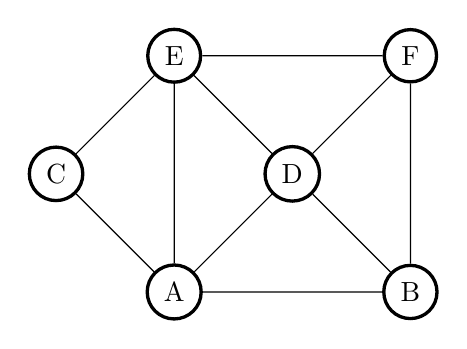
\begin{tikzpicture}
                     [scale=1.5,auto=left,every node/.style={circle,draw, very thick}]
                     \node (a) at (1,0)  {A};
                     \node (b) at (3,0)  {B};
                     \node (c) at (0,1)  {C};
                     \node (d) at (2,1)  {D};
                     \node (e) at (1,2)  {E};
                     \node (f) at (3,2)  {F};
                    % \foreach \from/\to in {b/d, b/e, b/f, b/g, d/c, d/g, d/f, e/c,
                    % e/g, e/f, f/c, g/c, a/e, a/f}
                    %    \draw (\from) -- (\to);
                    % \draw[bend left] (a) to (d);
                    % \draw[bend right] (a) to (g);
                     \draw (b) -- (a) -- (c) -- (e) -- (f);
                     \draw (a) -- (d) -- (b) -- (f) -- (d) -- (e) --
                     (a);
                   \end{tikzpicture} 
              \end{center}
              Esse grafo possui $|V(G)| = 6$ e $|A(G)| = 10$. Portanto
              temos que 
              $$
               2|V(G)| = 12 = 10 + 2 = |A(G)| + 2 
              $$
              Mas note que esse grafo não é auto-dual. Os vértices $E$,
              $A$ e $D$ possuem grau $4$. Entretanto, nenhuma face de
              $G$ possui grau $4$, e portanto, nenhum vértice de $G^*$
              terá grau $4$. Portanto, $G$ e $G^*$ não podem ser
              isomorfos e $G$ não é auto-dual.
    \end{enumerate}
    \paragraph{E42.} Para todo par $u,v$ de vértices de um grafo, seja
    $\gamma(u,v)$ a cardinalide de uma \textit{coleção máxima} de
    caminhos de $u$ a $v$, dois a dois internamente disjuntos (nos
    vértices), cada um de comprimento pelo menos 2.\medskip\newline
    Prove que se $G$ é um grafo tal que $\gamma(u,v) \leq 2$ para todo
    par $u,v \in V(G)$, etnão $G$ é planar.

    \paragraph{Solução:}
    Para essa questão iremos prova primeiro a seguinte
    afirmação:
    \paragraph{Lema Auxiliar: }Se $G$ é uma subdivisão de $K_5$ ou $K_{3,3}$ então existe um par
    de vértices $v, w \in V(G)$ tais que $\gamma(u,v) = 3$.
    \begin{proof}
        Seja $G$ um grafo que é subdivisão de $K_5$ ou $K_{3,3}$.Faremos a prova por indução em $k \geq 0$, onde $k$ é o número
        de vértices com grau 2 em $G$, ou seja, o número  operações de
        subdivisão apicadas a $K_5$ ou $K_{3,3}$ que originam o grafo $G$.\newline
        \textbf{Base:} Suponha $k = 0$. Então $G$ é $K_5$ ou $K_{3,3}$
        em ambos os casos, existem 2 vértices $v,w\in V(G)$, tais que
        existem 3 caminhos distintos com comprimento maior que 2 e disjuntos nos vértices que ligam
        ambos.\newline
        \textbf{Passo:} Suponha $k\geq 1$ e que a afirmação vale
        para grafos originados com $k-1$ operações de subdivisão.
        Seja $i \in V(G)$ um vértice de grau 2, ou seja,
        originado por uma operação de subdivisão e seja $j$ um vizinho
        qualquer de $i$. Defina $G'=G/ij$ e seja $z$ o vértice
        originado da contração das arestas $i$ e $j$. Então $G'$ possui
        exatamente $k-1$ vértices com grau 2 e também é uma
        subdivisão de $K_5$ ou $K_{3,3}$ pois a operação de
        contração foi aplicado à uma aresta originada por uma
        subdivisão. Então, por hipótese, existem dois vértices $u,v \in
        V(G)$ que possuem 3 caminhos $C_1, C_2, C_3$ disjuntos nos vértices de
        tamanho pelo menos 2.\newline
        Se $z$ não pertence a nenhum desses caminhos então os 3 caminhos
        também são 3 caminhos disjuntos e de tamanho 2 em G.\newline
        Caso contrário, sem perda de generalidade, suponha que
        $z\in C_1$. Então $C_1 = (u = v_1, \dots, z, \dots, v = v_l)$.
        Defina $C' = (u = v_1, \dots, i, j, \dots, v = v_l) $.$C'$
        possui comprimento maior que $C_1$ e os novos vértices
        utilizados não estão presentes nos outros caminhos $C_2$ e $C_3$ Assim
        temos que $C_2, C_3, C'$ são 3 caminhos disjuntos nos vértices e
        de tamanho pelo menos 2 para os vértices $u,v$ em $G$.\par
        Portanto, pelo princípio da indução, a afirmação vale.
    \end{proof}

    Agora para a prova pedida:

    \begin{proof}
        Seja $G$ um grafo tal que $\gamma(u,v) \leq 2$ para todo $u,v
        \in V(G)$. Como $\gamma(u,v) \leq 2$ para todo $u,v \in V(G)$
        então, pelo \textbf{Lema Auxiliar} $G$ não possui subdivisões de
        $K_5$ e $K_{3,3}$ e portanto, pelo \textbf{Teorema de
        Kuratowski} o grafo $G$ é planar.
    \end{proof}

\end{document}
